\chapter{Machine Learning and Classification Methods}
\label{chapter: Machine Learning and Classification Methods}


\section{Machine Learning}
Machine learning is a branch of computer science that deals with building and analyzing systems that are able to learn from data. Algorithms based on such analysis involve constructing a model from a given dataset, and then using this model to perform required tasks. Machine learning techniques can broadly be divided into two categories - supervised learning, and unsupervised learning.

\begin{itemize}
    \item{\textbf{Supervised Learning} Methods falling in this category operate in two phases. In the first step, the availability of training data is assumed, which is used to build a model so that it takes into account the structure of the given dataset. In the second step, this model is used to make predictions on the testing data (the real world data). This is the data that the model has not seen yet, and is required to make predictions on.}
    \item{\textbf{Unsupervised Learning} Methods falling under this category operate in a single phase. It starts with a model with zero knowledge about the structure of the given dataset. As data is fed into the model, it continuously learns the structure of the given dataset and calculates the predictions based on this knowledge. The main difference between this family of algorithms and supervised learning algorithms is the presence/absence of training labels.}
\end{itemize}

The primary focus in this thesis remains on supervised learning methods.\\

\section{Classification Methods}
Text classification is a subset of machine learning algorithms used to assign specific categories to pieces of data. It is one of the msot fundamental problems in machine learning. More precisely, given some sample information (such as what kind of data points are to be assigned to which category), these algorithms allow for assigning categories to unseen data points. Under the scope of this thesis, the data is always assumed to be English-text. Since machine learning algorithms only deal with real numbers, a necessary first step is the conversion of natural language text into real numbers. The work presented in this thesis makes extensive use of supervised text classification algorithms.\\

Given a dataset $\mathbf{X}$, it is required to separate the samples contained within the dataset into two (or more than two, depending on the input) classes. Formally, given a dataset that contains $N$ instances,

\begin{center}
    $\{(x_n, y_n)\}_{n = 1}^{N}$,
\end{center}

where each instance ($x_n, y_n$) is of the form,

\begin{center}
    $[(x_{n, 1}, x_{n, 2}, ... x_{n, D}), y_{n}]$,
\end{center}

each $x_{n, d}$ being the value of the feature $d \in [1, D]$, and $y_n$ being the label of the sample which can take a limited number of possible values, the aim is to calculate the value of $y_n$ given this feature information. In the supervised learning problem, this dataset is divided into two parts - training data (which contains the $y_n$ values for each instance), and test data (no information on $y_n$ is available), and the problem is to identify the values of $y_n$ in the test data given only the information present in the training data. On the other hand, in unsupervised text classification, the model is required to identify the $y_n$ values given only the values for $x_n$, there being no distinction between training and test data.\\

The performance of a particular classifier varies with the type of the data to be classified. Not all classifiers are good for all classes of problems. Some classifiers suit a particular problem more than some others; choosing a classifier for a problem still remains a decision which may or may not be completely scientific, even though a lot of work has been done to correlate classifier performance with data type.

\section{Support Vector Machines}
Support Vector Machines (SVMs) form a fairly popular class of machine learning algorithms used mainly for binary classification and regression analysis. Given the training data, the goal of an SVM is to find a decision boundary (a hyperplane in a high or infinite dimensional space) that separates the two classes of data while maximizing the distance of the boundary from any data point. The resulting decision function is fully specified by a (usually small) subset of the data, and the points in this subset are referred to as support vectors.\\

Most classifiers resort to a distance function, in some form or the other, that can provide a similarity measurement between two points. In the simplest form of an SVM, the distance function is simply the dot product between two points, and such SVMs are referred to as \emph{Linear Support Vector Machines}. In the case that a simple linear SVM is not able to find a sufficiently accurate decision boundary that can separate the data points into two classes (simply because the input data is not linearly separable), the so-called \emph{kernel trick} is used, which involves transforming the data from a low dimensional space to a much higher dimensional feature space (in which the input data may be separable) using an appropriate function

\begin{center}
    $\phi(x): \mathbb{R}^{L} \rightarrow \mathbb{R}^H (L \ll H)$
\end{center}

and then using the kernel function $\mathbf{k(\phi(x), \phi(y))}$ to actually perform the separation. The trick involved is that even though the transformation $\phi(x)$ may be expensive, computing the final similarity value $\mathbf{k(\phi(x), \phi(y))}$ is not.\\

Some of the most popular kernel functions include
\begin{itemize}
    \item{Linear (the simple SVM) - $k(x, y) = (x \cdot y)$ }
    \item{Polynomial - $k(x, y) = (\gamma x \cdot y + c)^{d}$}
    \item{Radial Basis - $k(x, y) = \exp(-\gamma {| x - y |}^{2})$}
    \item{Sigmoid - $k(x, y) = \tanh(\gamma x \cdot y + c)$}
\end{itemize}

Figure~\ref{fig:svm_linear_classify} shows a scenario where a support vector machine is used to classify two sets of points that are generated from partially overlapping Gaussian distributions. This dataset can be classified by a linear kernel SVM since this data is linearly separable.\\

\begin{figure}[t!]
    \centering
    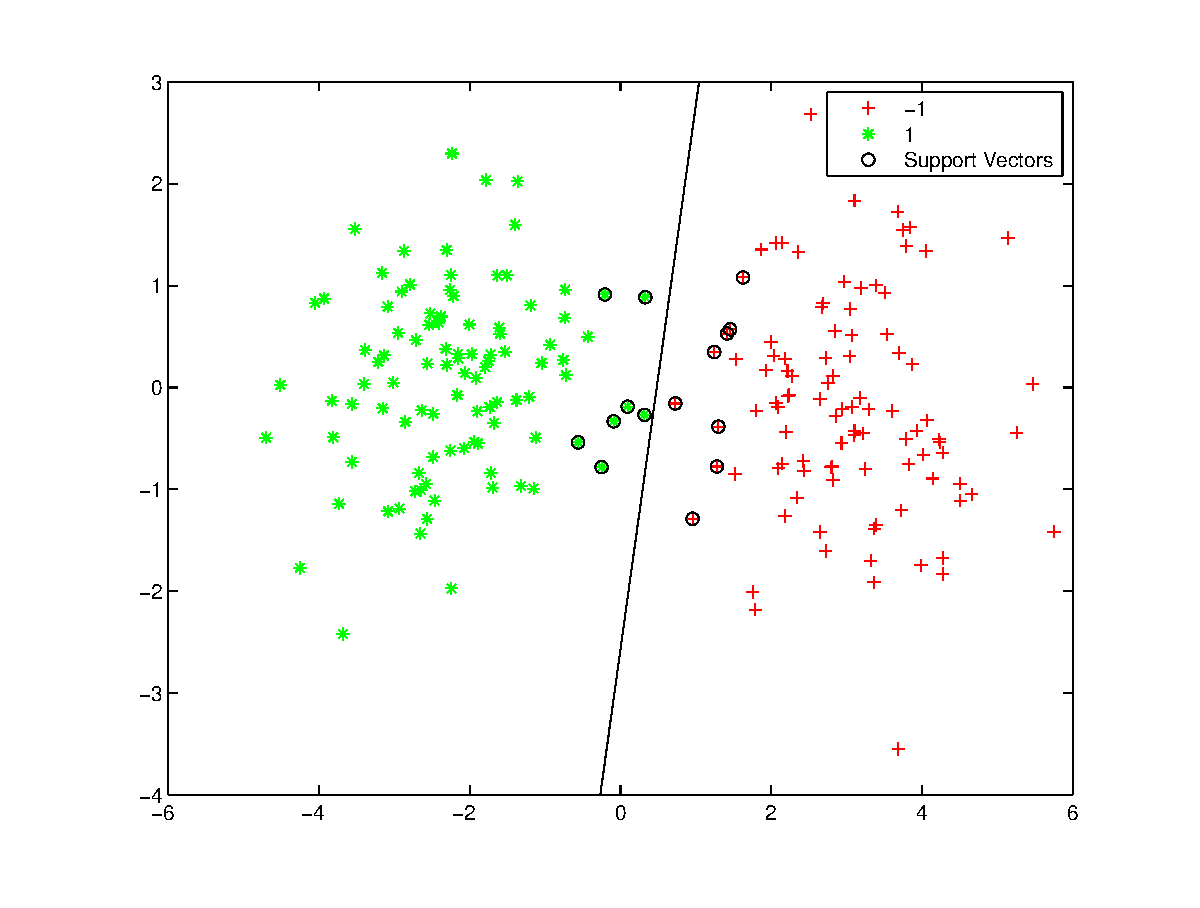
\includegraphics[width=0.8\textwidth]{svm_linear_classification.eps}
    \caption{Classification using a linear kernel SVM}
    \label{fig:svm_linear_classify}
\end{figure}

However, for a case when the data is not linearly separable and looks like as shown in Figure~\ref{fig:svm_non_linear_data}, the linear kernel performs poorly. This is shown in Figure~\ref{fig:svm_non_linear_classify_linear}. When the dataset has such characteristics, a much better option is to use a kernel that is able to work with such data. For instance, an RBF kernel draws a much better boundary in this case, as shown in Figure~\ref{fig:svm_non_linear_classify_rbf}.\\

\begin{figure}[t!]
    \centering
    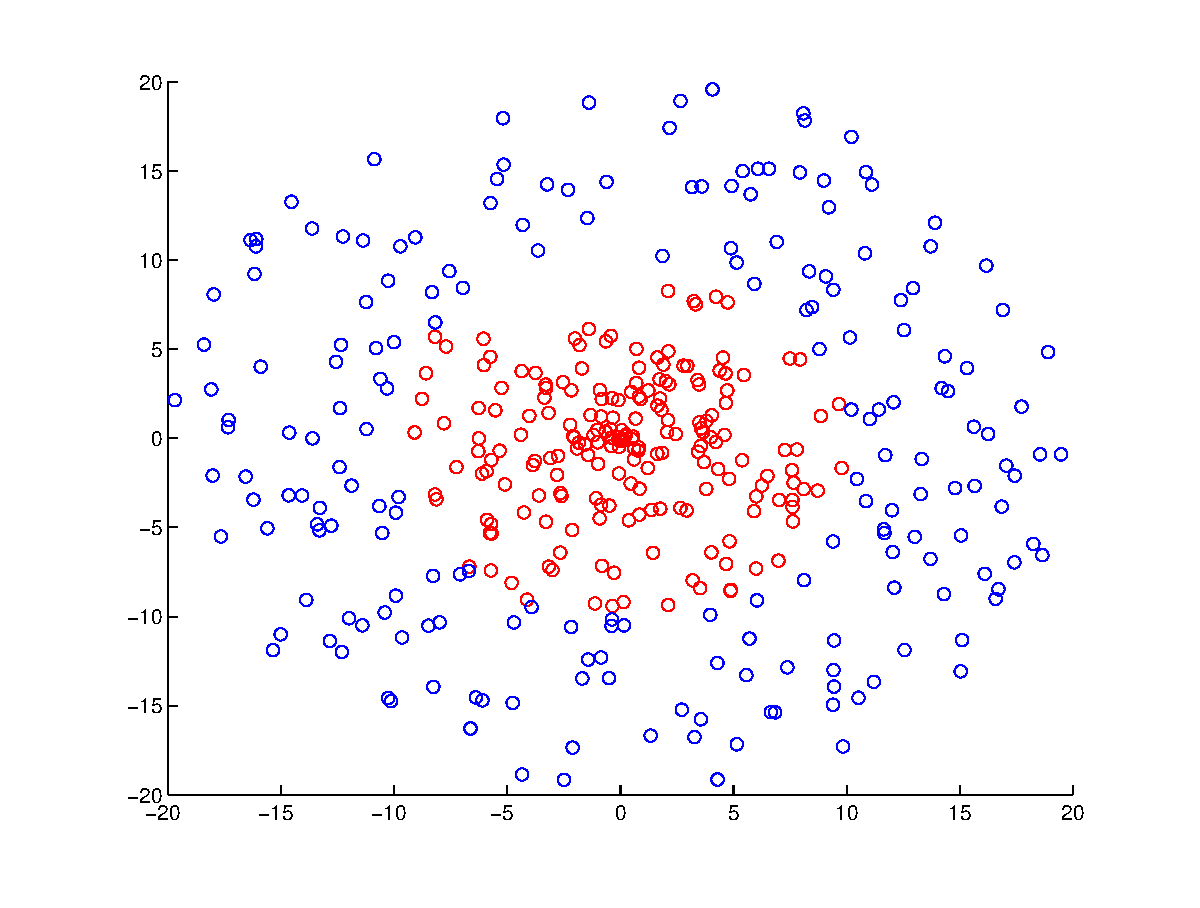
\includegraphics[width=0.8\textwidth]{svm_non_linear_data.eps}
    \caption{A dataset which is not linearly separable}
    \label{fig:svm_non_linear_data}
\end{figure}

\begin{figure}[t!]
    \centering
    \includegraphics[width=0.8\textwidth]{svm_non_linear_classify_linear.eps}
    \caption{Dataset for Figure~\ref{fig:svm_non_linear_data} being classified using a linear kernel}
    \label{fig:svm_non_linear_classify_linear}
\end{figure}

\begin{figure}[t!]
    \centering
    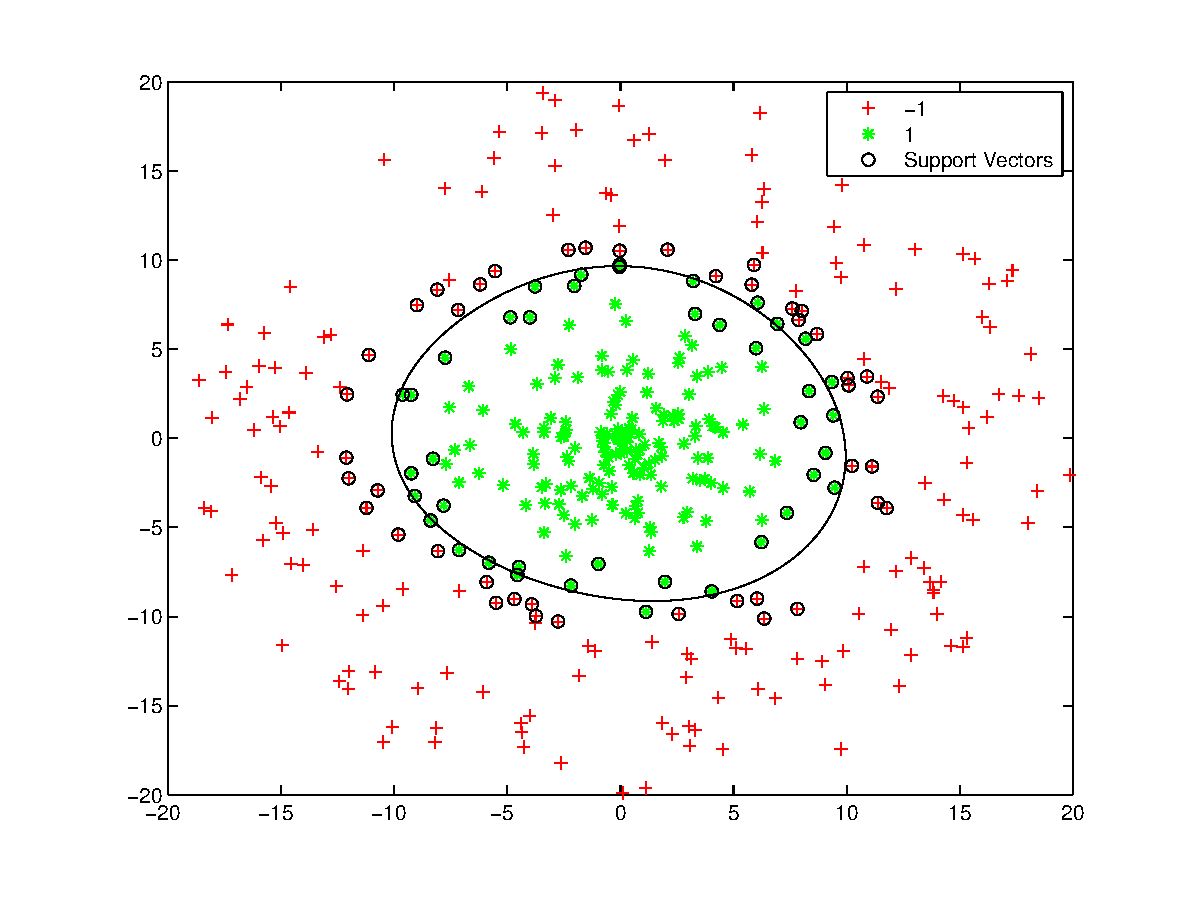
\includegraphics[width=0.8\textwidth]{svm_non_linear_classify_rbf.eps}
    \caption{Dataset for Figure~\ref{fig:svm_non_linear_data} being classified using an RBF kernel}
    \label{fig:svm_non_linear_classify_rbf}
\end{figure}

Intuitively, the work done by the $\phi(x)$ function can be visualized from Figure~\ref{fig:svm_non_linear_data}, and Figure~\ref{fig:svm_non_linear_data_3d}. Figure~\ref{fig:svm_non_linear_data} shows the original dataset that the linear kernel failed to classify with reasonable accuracy. A simple transformation can be applied in this case to make the data separable, transforming the two dimensional input to a three dimensional input by adding the following transformation.\\

\begin{center}
    $ \phi(x) = \sqrt{x_1^2 + x_2^2} $
\end{center}

This transformation transforms the input data in the shape of a three dimensional cone which is separated into two parts by a simple plane in three dimensions. The points in the inner circle form the tip and the surrounding areas of the cone, while the rest of the cone is constituted by the remaining points. The resulting data looks like Figure~\ref{fig:svm_non_linear_data_3d}.\\

\begin{figure}[t!]
    \centering
    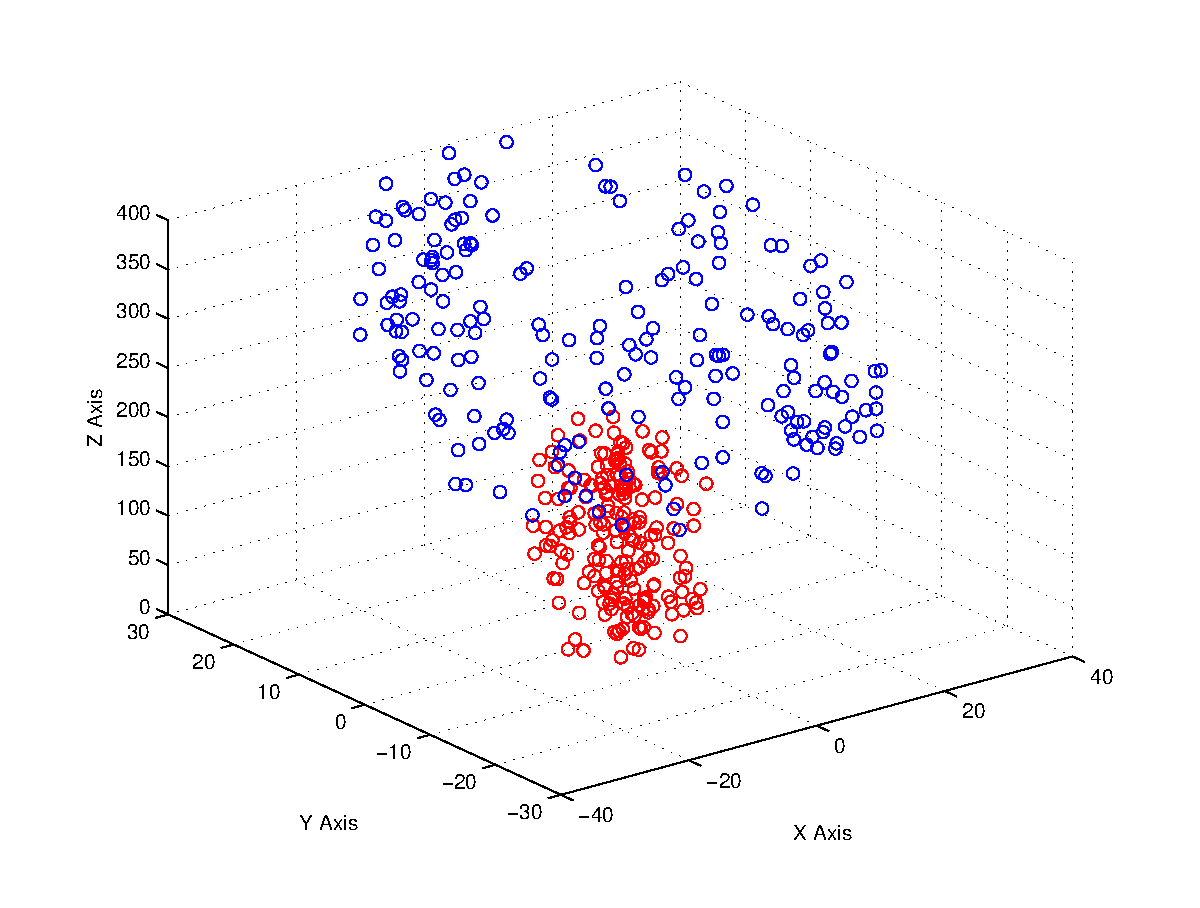
\includegraphics[width=0.8\textwidth]{svm_non_linear_data_3d.eps}
    \caption{The dataset from Figure~\ref{fig:svm_non_linear_data}, exported into a three dimensional space, which can now be separated by a linear plane}
    \label{fig:svm_non_linear_data_3d}
\end{figure}

The code for this transformation (including the generation of the original data) is shown in Listing~\ref{lst:svm_linear_classify}.\\

\lstinputlisting[language=Matlab,caption={Generating the dataset to be classified by a linear classifier},label={lst:svm_linear_classify}]{code/svm_linear_classify.m}
